\documentclass[a4paper,12pt]{report}
\usepackage[left=0.75in,right=0.75in,top=1.0in,bottom=1.5in,footskip=.25in]{geometry}
\usepackage[hidelinks]{hyperref}
\usepackage{graphicx}
\usepackage[english]{babel}
\usepackage[utf8]{inputenc}
\usepackage{url}
\usepackage[toc,acronym,section]{glossaries}
\usepackage[section]{placeins}


\usepackage[toc,page,header]{appendix}
\usepackage{hhline,colortbl,color,booktabs}
\usepackage{longtable}

\renewcommand\thesection{\arabic{section}}
\renewcommand\thesubsection{\arabic{subsection}.}
\renewcommand\thesubsubsection{\alph{subsubsection}}

\newcommand{\TermName}{SUMMER 2020}
\newcommand{\Course}{\textbf{SOEN-6471 \vspace{0.5cm} ADVANCED SOFTWARE ARCHITECTURES}}
\newcommand{\ProfessorName}{Dr. PANKAJ KAMTHAN}

\begin{document}

\begin{titlepage}

\newcommand{\HRule}{\rule{\linewidth}{0.5mm}} 

\centering
\textbf{\LARGE  } \\ [5mm] 

\includegraphics[scale=.2]{University_logo.jpg}\\[1cm] 
\textsc{\Large \Course (\TermName)} \\  [0.5cm]

	
\HRule \\[0.6cm]
{ \huge \bfseries iCARE}\\[0.4cm] 
\HRule \\[0.5cm]

{\large \textbf{DELIVERABLE 1 (D1)} }	

\HRule \\[1.5cm]

\vspace{3cm}

\begin{flushleft}


\textbf{\underline{\Large Submitted By: (Team D)}}
\hfill
\textbf{\underline{\Large Submitted To:}} \\
\vspace{3mm}
\large Niralkumar Lad(40080612)
\hfill
\large Dr. Pankaj Kamthan \\
\large Moshood Kolawole (40102157) \hfill \\
\large Ahmad Memari (40088010) \hfill \\
\large Xiaofeng Liu (40126183) \hfill \\
\large Anusha Keralapura Thandavamurthy (40102962) \\

\end{flushleft}

\centering \vspace{1cm}

$GitHub - \href{https://github.com/Anushakt/SOEN_6471_SoftwareArchitecture}{https://github.com/Anushakt/SOEN_6471_SoftwareArchitecture}$

\vfill
\end{titlepage}


\pagenumbering{roman}
\renewcommand*\contentsname{TABLE OF CONTENT}
\tableofcontents

\listoffigures

\newpage
\pagenumbering{arabic}
\addcontentsline{toc}{chapter}{PART 1: VISION}
\chapter*{PART 1: VISION}



\addcontentsline{toc}{section}{Project Overview}
\section*{Project Overview}
The iCare project is going to be solely implemented for patients, doctors and admin. In detail, the main function of the system is to register and select a doctor to make the appointment completely online. Patient will be able to access their appointment history and make/reschedule an appointment specific to their problem through the web app.
\addcontentsline{toc}{section}{Project Background}
\section*{Project Background}
With the COVID-19 pandemic in 2020, Health Informatics is becoming more important than ever.Online Appointment System can greatly improve patients' experience as well as reducing the workload on doctors and medical system.
 
\addcontentsline{toc}{section}{Busines Goal} 
\section*{Business Goal}
To design and develop an Online Booking Appointment for iCare which allows a potential patient to book an appointment with the doctor directly through the website.The system will:
\begin{enumerate}
\item Be accessible on any mobile device with an internet connection within Canada.
\item Reduce the workload on medical system staffs greatly.
\item Visualize the appointment schedule so that it is easy to manage appointments and make the workflow less cluttered.
\item Offer patients greater choice and convenience, and remove the opportunity for double-bookings.
\item Design and implement the appointment list so that it is easy to manage appointments and make the workflow less cluttered.
\item Improve data capturing and reporting.
    
\end{enumerate}

\addcontentsline{toc}{chapter}{PART 2: STAKEHOLDERS AND CONCERNS}
\chapter*{PART 2: STAKEHOLDERS AND CONCERNS}

\addcontentsline{lof}{section}{Mind Map}
\addcontentsline{toc}{section}{Mind Map}
\section*{ Mind Map:}

\begin{center}
    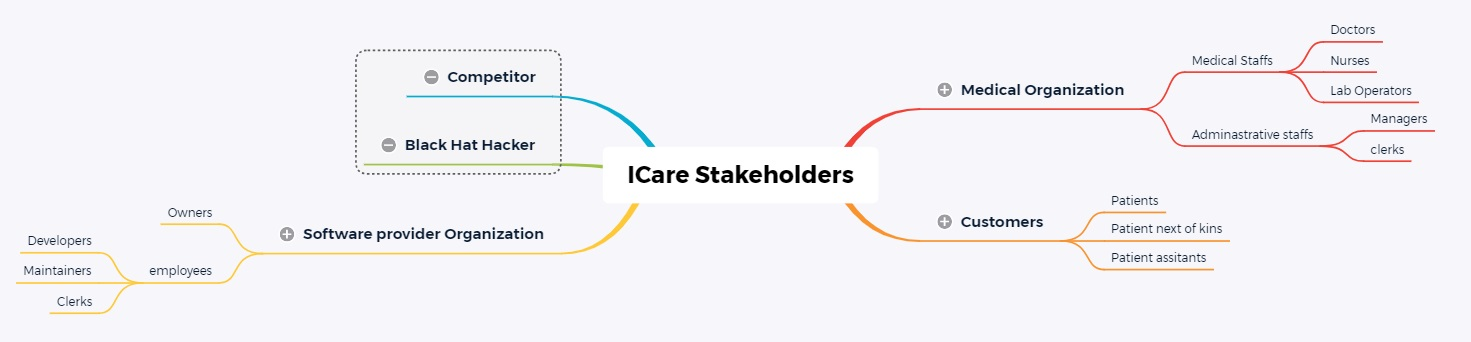
\includegraphics[scale=0.7]{MindMap.jpg}\\
    \textbf{Mind Map}
\end{center}


\addcontentsline{toc}{section}{List of Stakeholders}
\section*{List of Stakeholders:}
\begin{enumerate}
    \item Software Provider Organization:
        \begin{enumerate}
            \item Owner.
            \item Employees:
                \begin{itemize}
                    \item Developers.
                    \item Maintainers.
                    \item Clerks.
                \end{itemize}
        \end{enumerate}
    \item Medical Organisation:
        \begin{enumerate}
            \item Medical Staff:
                \begin{itemize}
                    \item Doctors.
                    \item Nurse.
                    \item Lab Operators.
                \end{itemize}
            \item Administrative Staff:
                \begin{itemize}
                    \item Managers.
                    \item Clerks.
                \end{itemize}
        \end{enumerate}
    \vspace{1mm}
    \item Customer:
        \begin{enumerate}
            \item Patient.
            \item Patient next of kin.
            \item Patient assistant.
        \end{enumerate}
    \item Black Hat Hacker.
    \item Competitor.
\end{enumerate}

\addcontentsline{toc}{section}{Concern}
\section*{Concerns:}
\begin{enumerate}
    \item \textbf{Patient:} They want to book appointments with doctor before visiting the clinic.
    \item \textbf{Doctor:} They want to view and follow-up appointments with their patients, create and update their patient's records from anywhere easily.
    \item \textbf{Receptionist/Administrator:} They want to register new patients and make changes to patients' information from anywhere.
\end{enumerate}

\addcontentsline{toc}{chapter}{PART 3: PROBLEM}
\chapter*{PART 3: PROBLEM}
\addcontentsline{toc}{section}{Functional Requirements}
\section*{Functional Requirements:}
\begin{enumerate}
    \item When the user, i.e. patient, doctor or admin, will try to login with the username and password, the system will match the credentials with those in the database and grant access to the system and display the dashboard if the credentials are valid and if the credentials are invalid, an appropriate message will be displayed.
    
    \item When the patient have logged in and when the patients click on the ‘Doctor Profile’ button on dashboard to view doctor’s profile, the system will show a list of all profile of the doctors available in the database. Here, the patient can click on the ‘Filter’ button to view the doctor’s profile based on doctor’s field of expertise as well as name.
    
    \item While on dashboard, when the patients click on ‘Book Appointment’ button, the system will show a list of available date and time-slots of the available doctors. 
    
    \item Further, to book an appointment, the patient shall have to select a time-slot for a particular doctor and confirm the appointment to which the system will prompt the user to again confirm the appointment to avoid any confusion or mistake.
    
    \item When the patient successfully book an appointment with a doctor, an email notification as well as a notification within the system will be send to the doctor and the patient. 
    
    \item When patient will be logged in and when they are on the dashboard, patient will be able to view the timeline which will depict written prescription by the doctor, the medical reports as well as the treatment plan.
    
    \item While the patient have logged in and when the patient clicks on ‘My Profile’ button, they will be able to see their respective profile and can update their profile, if necessary.
    
    \item When the doctors have logged in and they click on ‘Patient Profile’ button on the dashboard, doctor will be able to view patient’s profile who are consulting them. 
    
    \item While viewing patients’ profile, if the doctor select any particular patient’s profile then the doctor will be able to enter new details about that specific patient’s health if there is none or the doctor will be able to update the details. To save the details, the doctor will have to confirm the details when prompted.
    
    \item When the doctor logged in and when they click on ‘View Appointments’ button on the dashboard, doctor will be able to view all the appointments of the patients who are consulting them in Chronological order.
    
    \item When the doctor is logged in and on the view appointment page, they can select and reschedule any appointment and that patient will be notified about the event.
    
    \item When the patient have logged in and when they click on ‘View Appointments’ button on the dashboard, they will be able to view upcoming appointments. 
    
    \item The patient will also be able to reschedule an appointment by clicking on the ‘Reschedule Appointment’ on the view appointment page but only with staff’s or doctor’s approval and the patient will receive the notification.
    
    \item When a user, i.e. patients accessing the system for the first time, then they will have to click on 'Sign Up' to create an account before they are able to access the system facilities but the staff will be registered into the system by the admin.
    
    \item When a user are on sign up page, they will have to fill up the mandatory details and click on 'Sign Up' button to continue using the system.
    
    
\end{enumerate}

\addcontentsline{toc}{section}{Non-Functional Requirements}
\section*{Non-Functional Requirements:} 
\begin{enumerate}
    \item Maintainability:
        \begin{enumerate}
            \item A Database server to store and manage the data.
            \item Backing up the database to a backup server at every midnight to restore the data in an event of server failure.
            \item Logging every event to keep a track in text form.
            \item Managing timestamp every time the data is changed.
    \end{enumerate}
    \item Privacy:
        \begin{enumerate}
            \item Only authorized users can log in/sign up to the system.
            \item Patients data can only be viewed by concerned doctors.
            \item Only admin will have access to give authorization for the staff.
            \item Patient's personal and medical data is not shared with anyone.
            \item Any change in the patient's profile should be notified.
            \item Privacy of communication channels, input interfaces, and secure storage of sensitive data.
        \end{enumerate}
    \item Security:
        \begin{enumerate}
            \item Use encryption to avoid bots from booking.
            \item Register with Social Security Card check.
            \item Ensure the appointment can only be viewed and modified by the corresponding patient and doctor.
            \item Set expiration time when users no longer use the website.
        \end{enumerate}
    \item Usability:
        \begin{enumerate}
            \item Giving a positive experience to the user.
            \item User should be guided for all process to complete all tasks required by the user.
            \item Minimize the need to have a tutorial to use the system.
            \item Easy to remember, rapid recovery from error and increasing productivity and profitability.
            \item Converting the maximum number of visitors of the system to clients.
            \item Different sign up/login for different categories of users.
            \item Sitemap to help user find the related information easily.
        \end{enumerate}
\end{enumerate}

\addcontentsline{toc}{chapter}{PART 4: VIEWPOINTS AND VIEW}
\chapter*{PART 4: VIEWPOINTS AND VIEW}

\addcontentsline{lof}{section}{4+1 View}
\begin{center}
    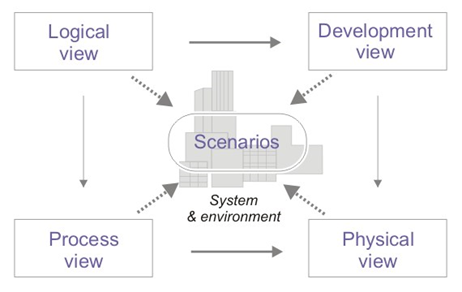
\includegraphics{UML/4view.png}\\
    \textbf{4+1 View}
\end{center}

\addcontentsline{toc}{section}{Logical View}
\section*{Logical View:}
The logical view is concerned with the functionality that the system provides to end-users. UML Diagrams used to represent the logical view include Class diagram, and interaction diagrams (communication diagrams, or sequence diagrams). Icare website allows the end user to book an appointment with doctors and share their health concerns with them. Another functionality is that the doctor can accept/reject the appointment and give suggestions to the patient by updating their profile.\\\\
\textbf{Stakeholders:} Designers.\\ 
\textbf{Representation:} Package Diagram.

\addcontentsline{lof}{section}{Package Diagram}
\begin{center}
    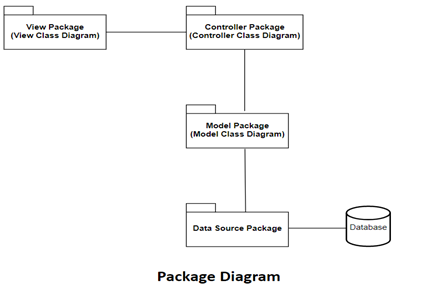
\includegraphics{UML/package.png}    
\end{center}

\addcontentsline{toc}{section}{Implementation View}
\section*{Development View or Implementation View:}
The development view illustrates a system from a programmer's perspective and is concerned with software management. This view is also known as the implementation view. It uses the UML Component diagram to describe system components.\\\\
\textbf{Stakeholders:} Programmers.\\
\textbf{Representation:} Package diagram, Component diagram

\begin{center}
    \addcontentsline{lof}{section}{Component Diagram}
    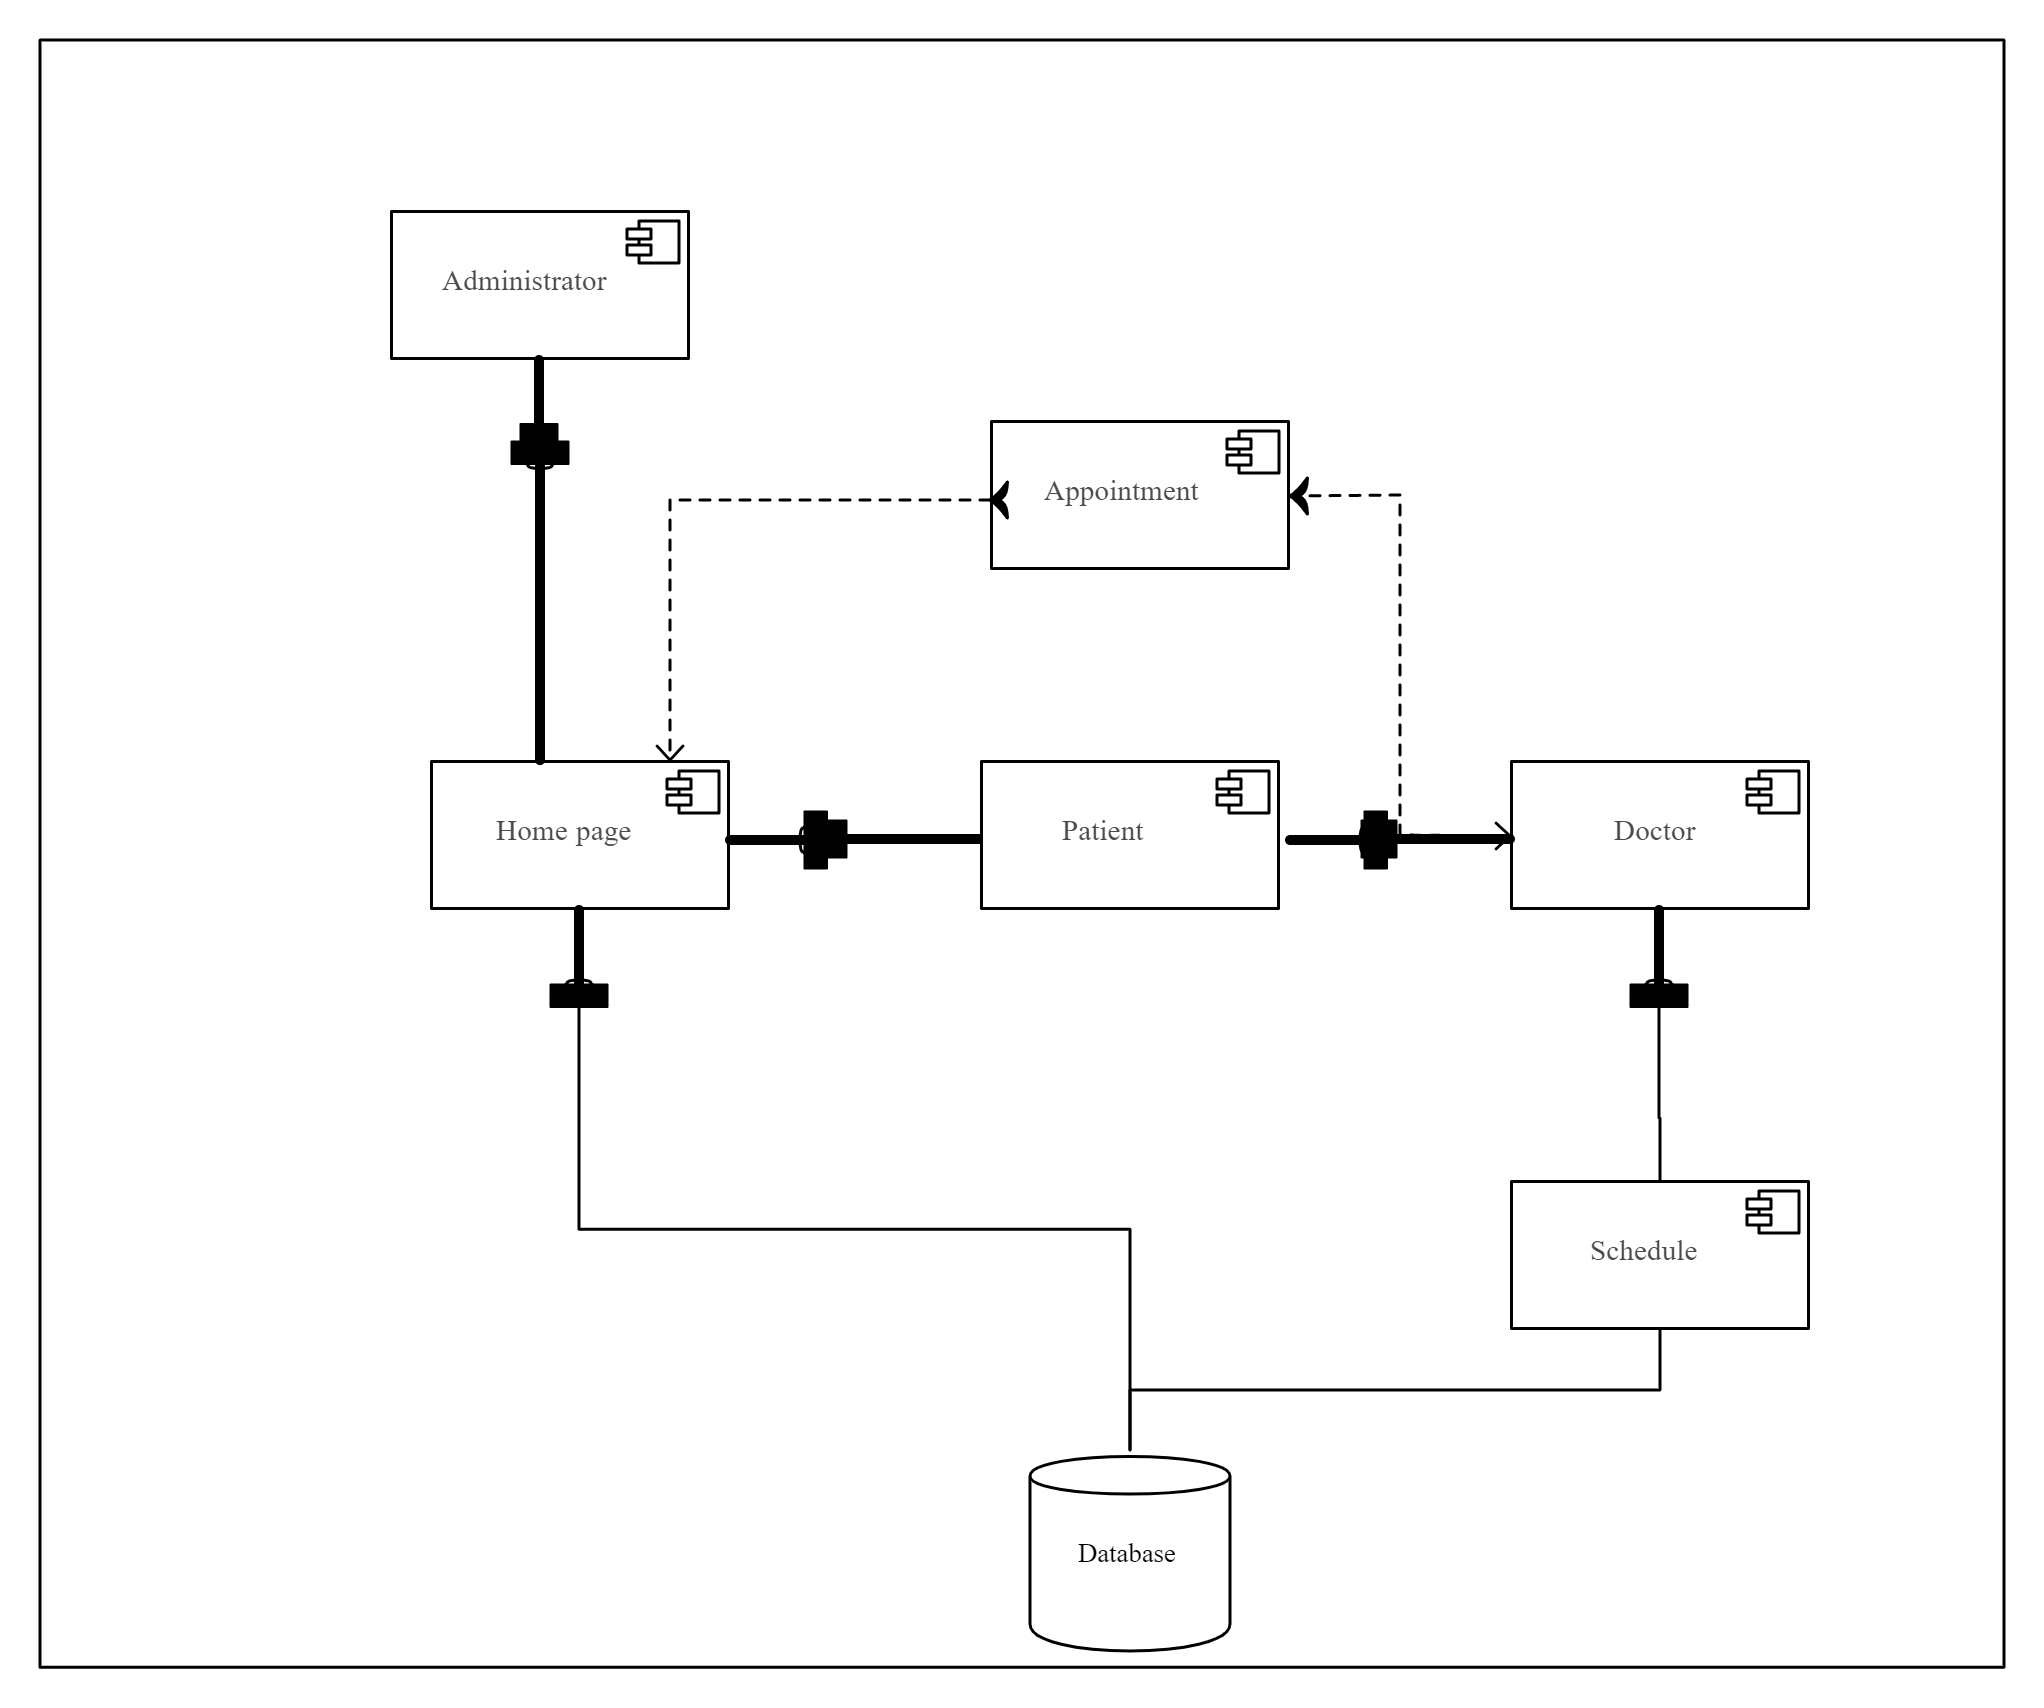
\includegraphics[scale=0.15]{UML/component.png}\\
    \textbf{Component Diagram}
\end{center}

\addcontentsline{toc}{section}{Process View}
\section*{Process view:}
The process view deals with the dynamic aspects of the system, explains the system processes and how they communicate, and focuses on the run-time behaviour of the system. The process view addresses concurrency, distribution, integrators, performance, and scalability and so on.\\\\
\textbf{Stakeholders:} Integrators\\
\textbf{Representation:} Class diagram and Interaction Diagram (Communication Diagram or Sequence Diagram)\\
\addcontentsline{lof}{section}{Class Diagram}
\begin{center}
        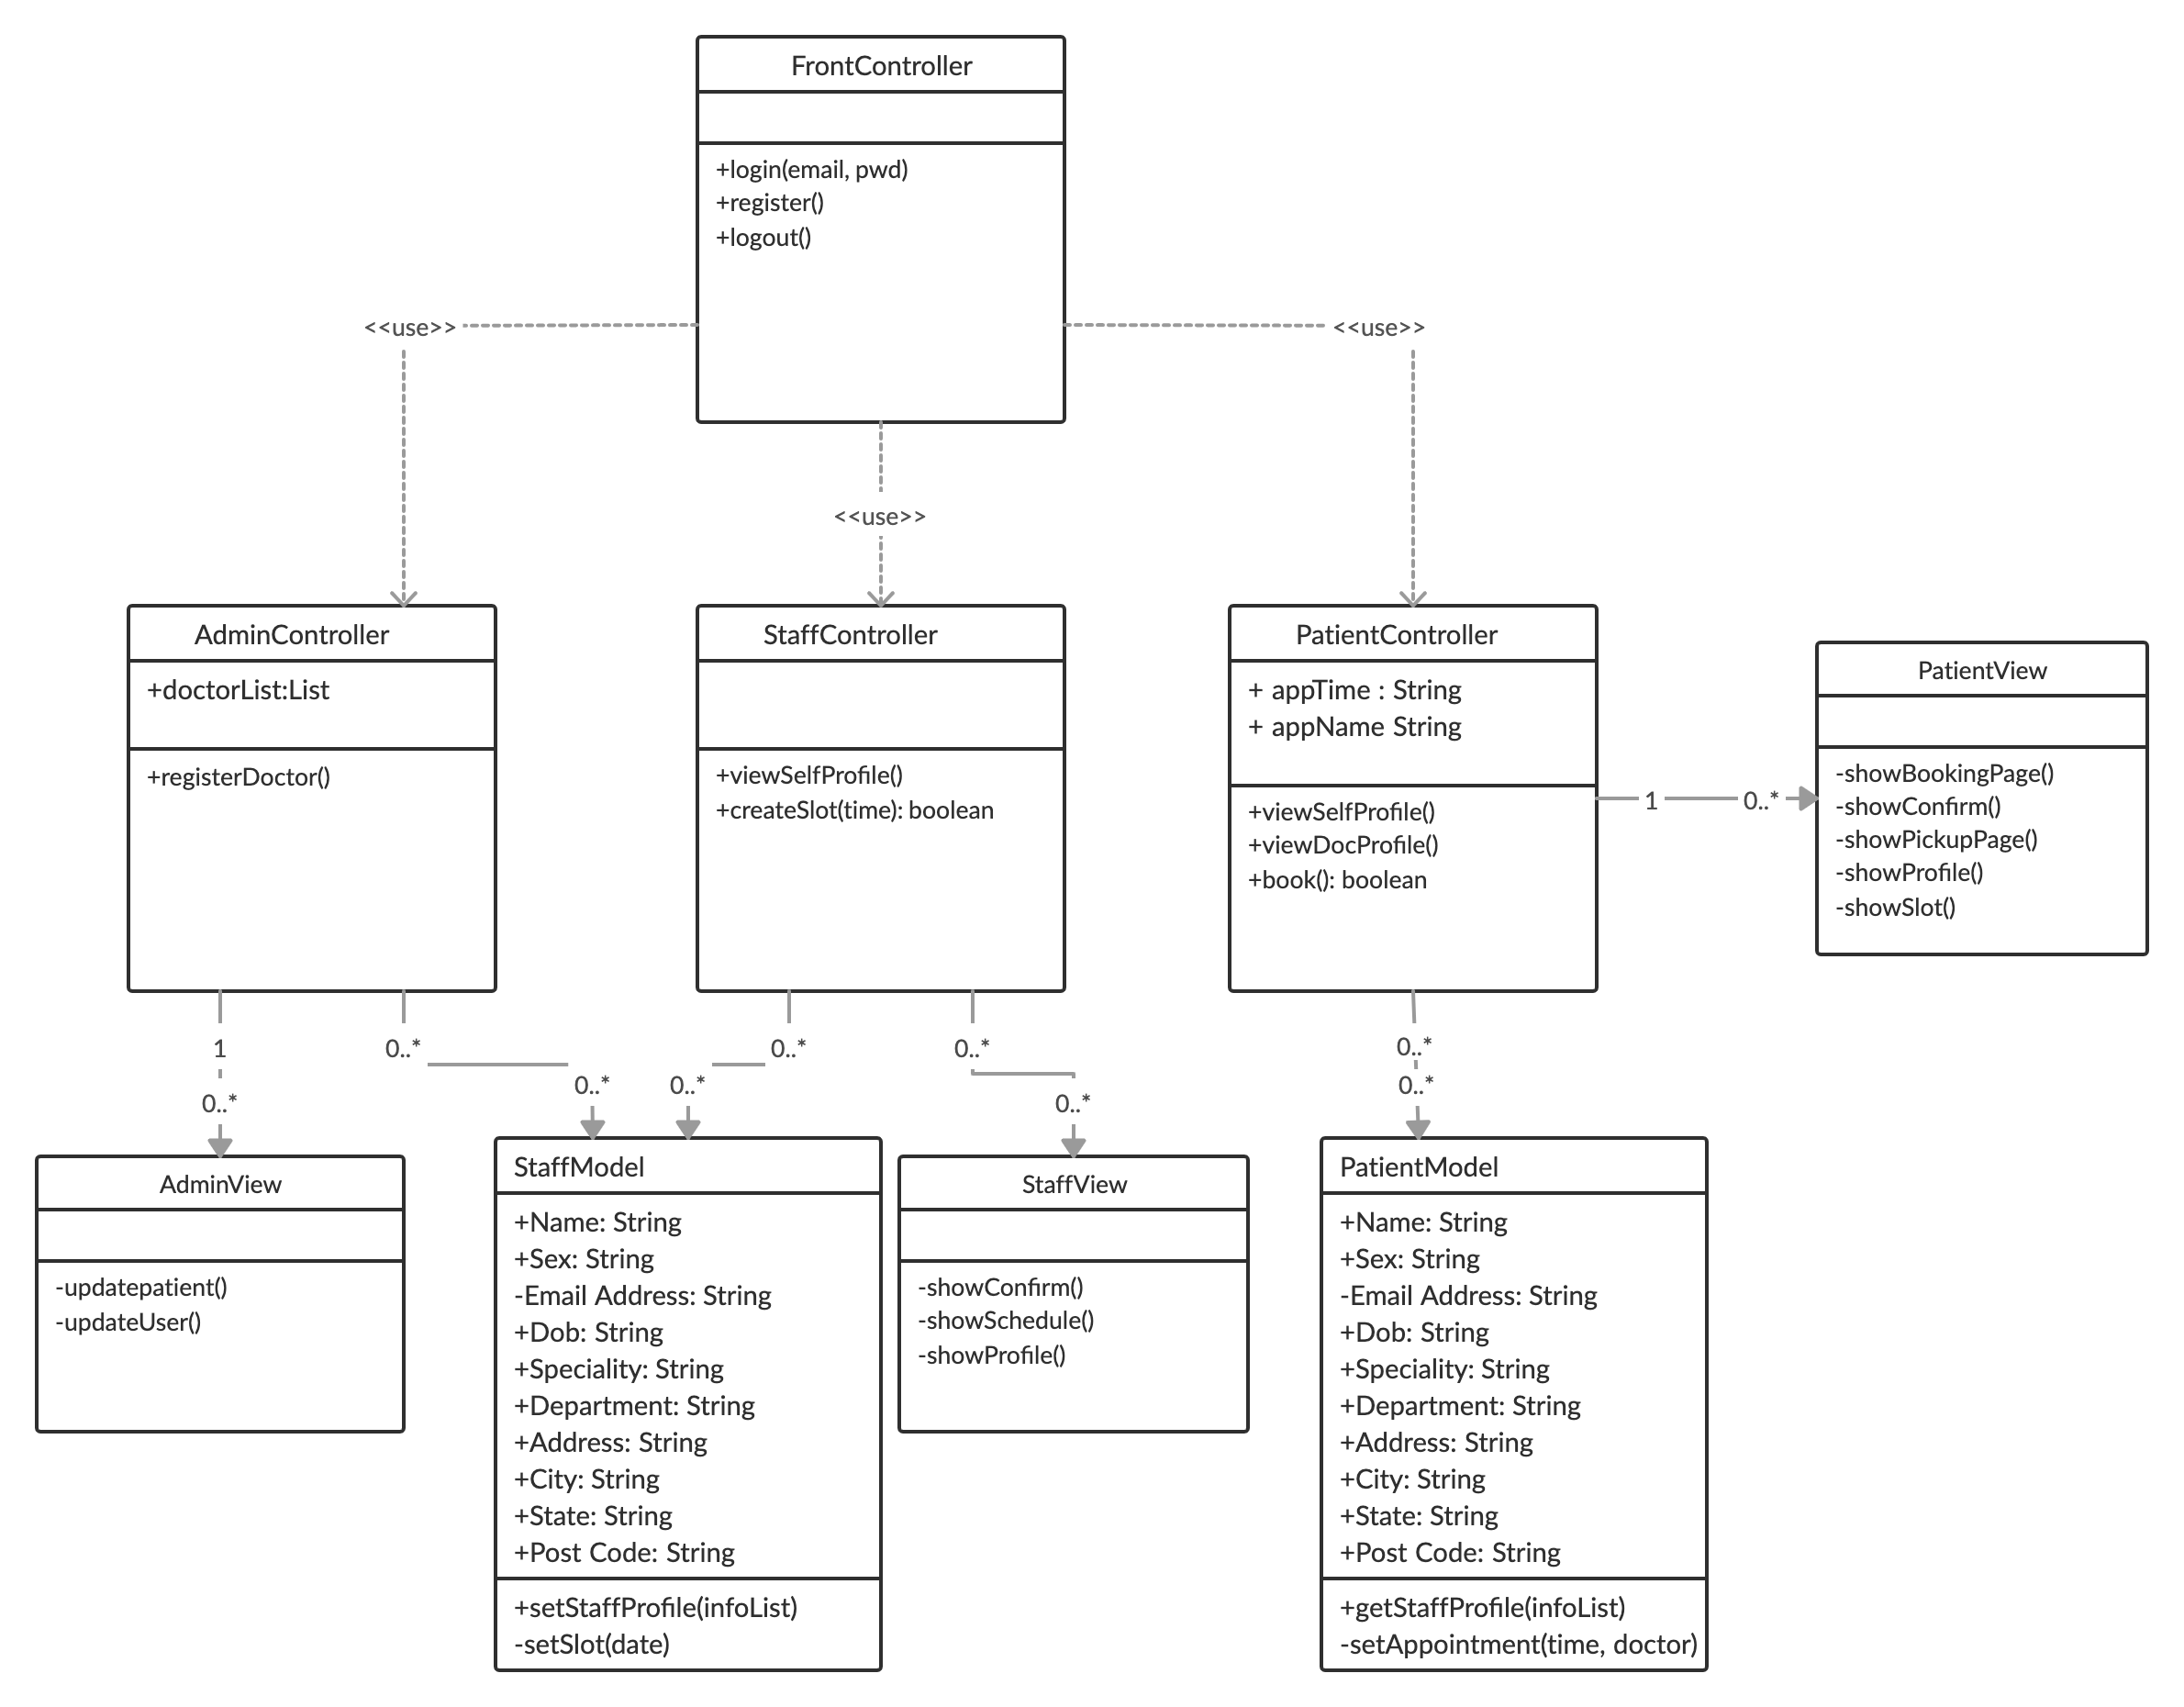
\includegraphics[scale=.2]{UML/class.png}\\
        \textbf{Class Diagram}
\end{center}
\vspace{0.5cm}    
The parts for Communication diagram are divided into 3 phases:
\vspace{0.5cm}
\begin{enumerate}
    \item \textbf{Patient Functionalities:} Book an appointment with a doctor.
        \begin{center}
            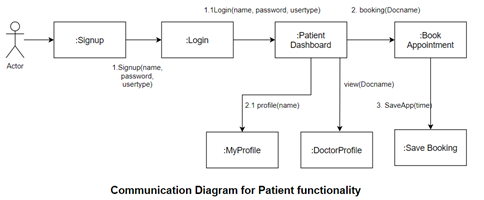
\includegraphics{UML/patient.png}    
            \addcontentsline{lof}{section}{Communication Diagram for Patient}
        \end{center}
    
    \item \textbf{Doctor Functionalities:} Schedule appointment and update patients’s profile.
    \addcontentsline{lof}{section}{Communication Diagram for Doctor}
        \begin{center}
            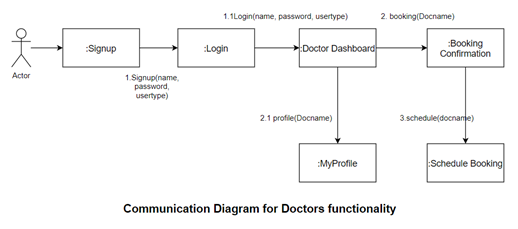
\includegraphics{UML/doctor.png}    
        \end{center}
        
    \item \textbf{Admin Functionalities:} To add and update user details.
    \addcontentsline{lof}{section}{Communication Diagram for Admin}
        \begin{center}
            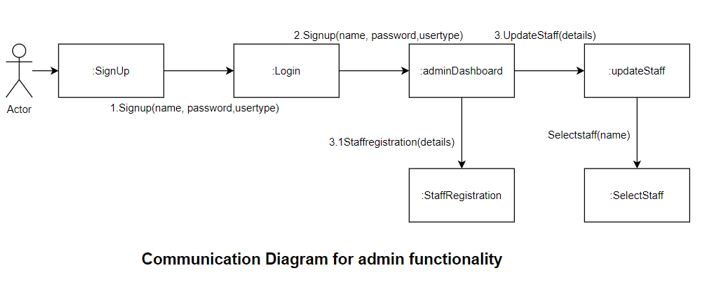
\includegraphics{UML/admin.JPG}
        \end{center}
\end{enumerate}

\begin{center}
    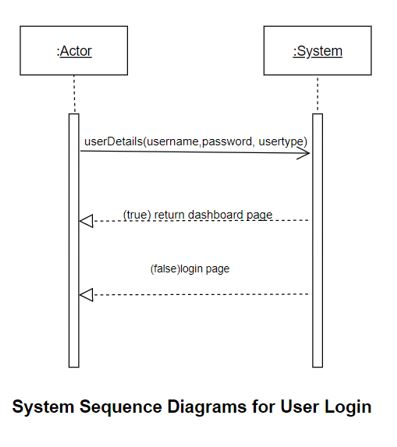
\includegraphics{UML/UserLogin.JPG}
    \addcontentsline{lof}{section}{User Login Sequence Diagram}
    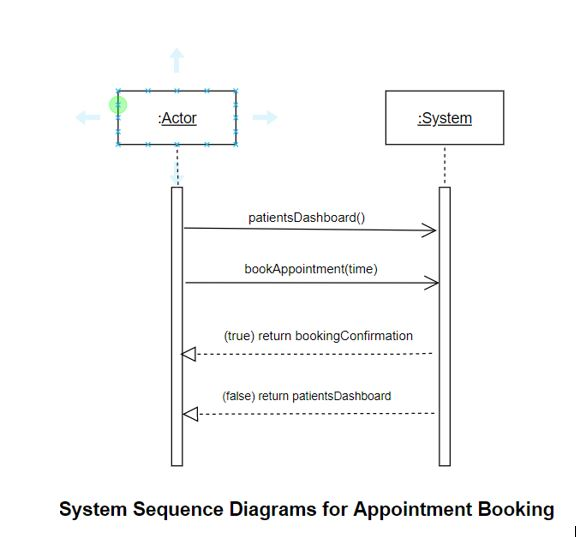
\includegraphics{UML/Appoinmentbooking.JPG}
    \addcontentsline{lof}{section}{Appointment Booking Sequence Diagram}
    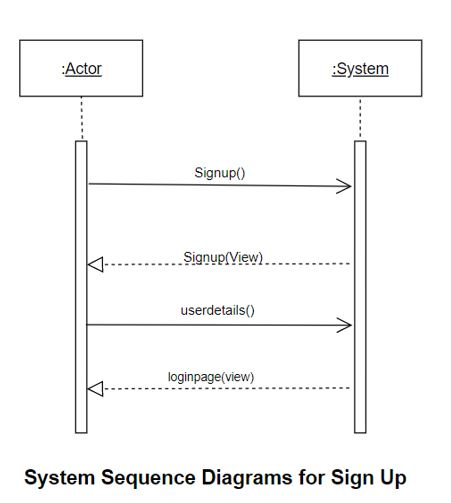
\includegraphics{UML/Signup.JPG}
    \addcontentsline{lof}{section}{Sign Up Sequence Diagram}
    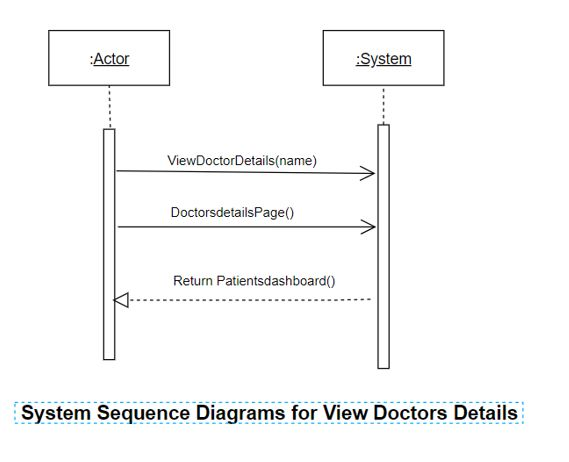
\includegraphics{UML/Viewdoctor.JPG}
    \addcontentsline{lof}{section}{View Doctor Details Sequence Diagram}
\end{center}


\addcontentsline{toc}{section}{Deployment View}
\section*{Physical or Deployment View:}
The physical view depicts the system from a system engineer's point of view. It is concerned with the topology of software components on the physical layer, as well as the physical connections between these components.\\\\
\textbf{Stakeholders:} Deployment managers and System Engineers.\\
\textbf{Representation:} Deployment diagram.

\begin{center}
    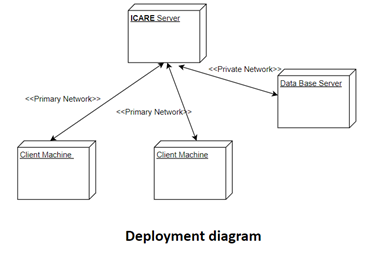
\includegraphics{UML/deployment.png}
    \addcontentsline{lof}{section}{Deployment Diagram}
\end{center}

\addcontentsline{toc}{section}{Use Case View}
\section*{Use Case View or Scenario View:}
The description of an architecture is illustrated using a small set of use cases, or scenarios which become a fifth view. The scenarios describe sequences of interactions between objects, and between processes. They are used to identify architectural elements and to illustrate and validate the architecture design. They also serve as a starting point for tests of an architecture prototype.\\\\
\textbf{Stakeholders:}All the stakeholders of the system, including the end-users.\\
\textbf{Representation:}Use-Case diagram, Activity diagram.
    \begin{center}
        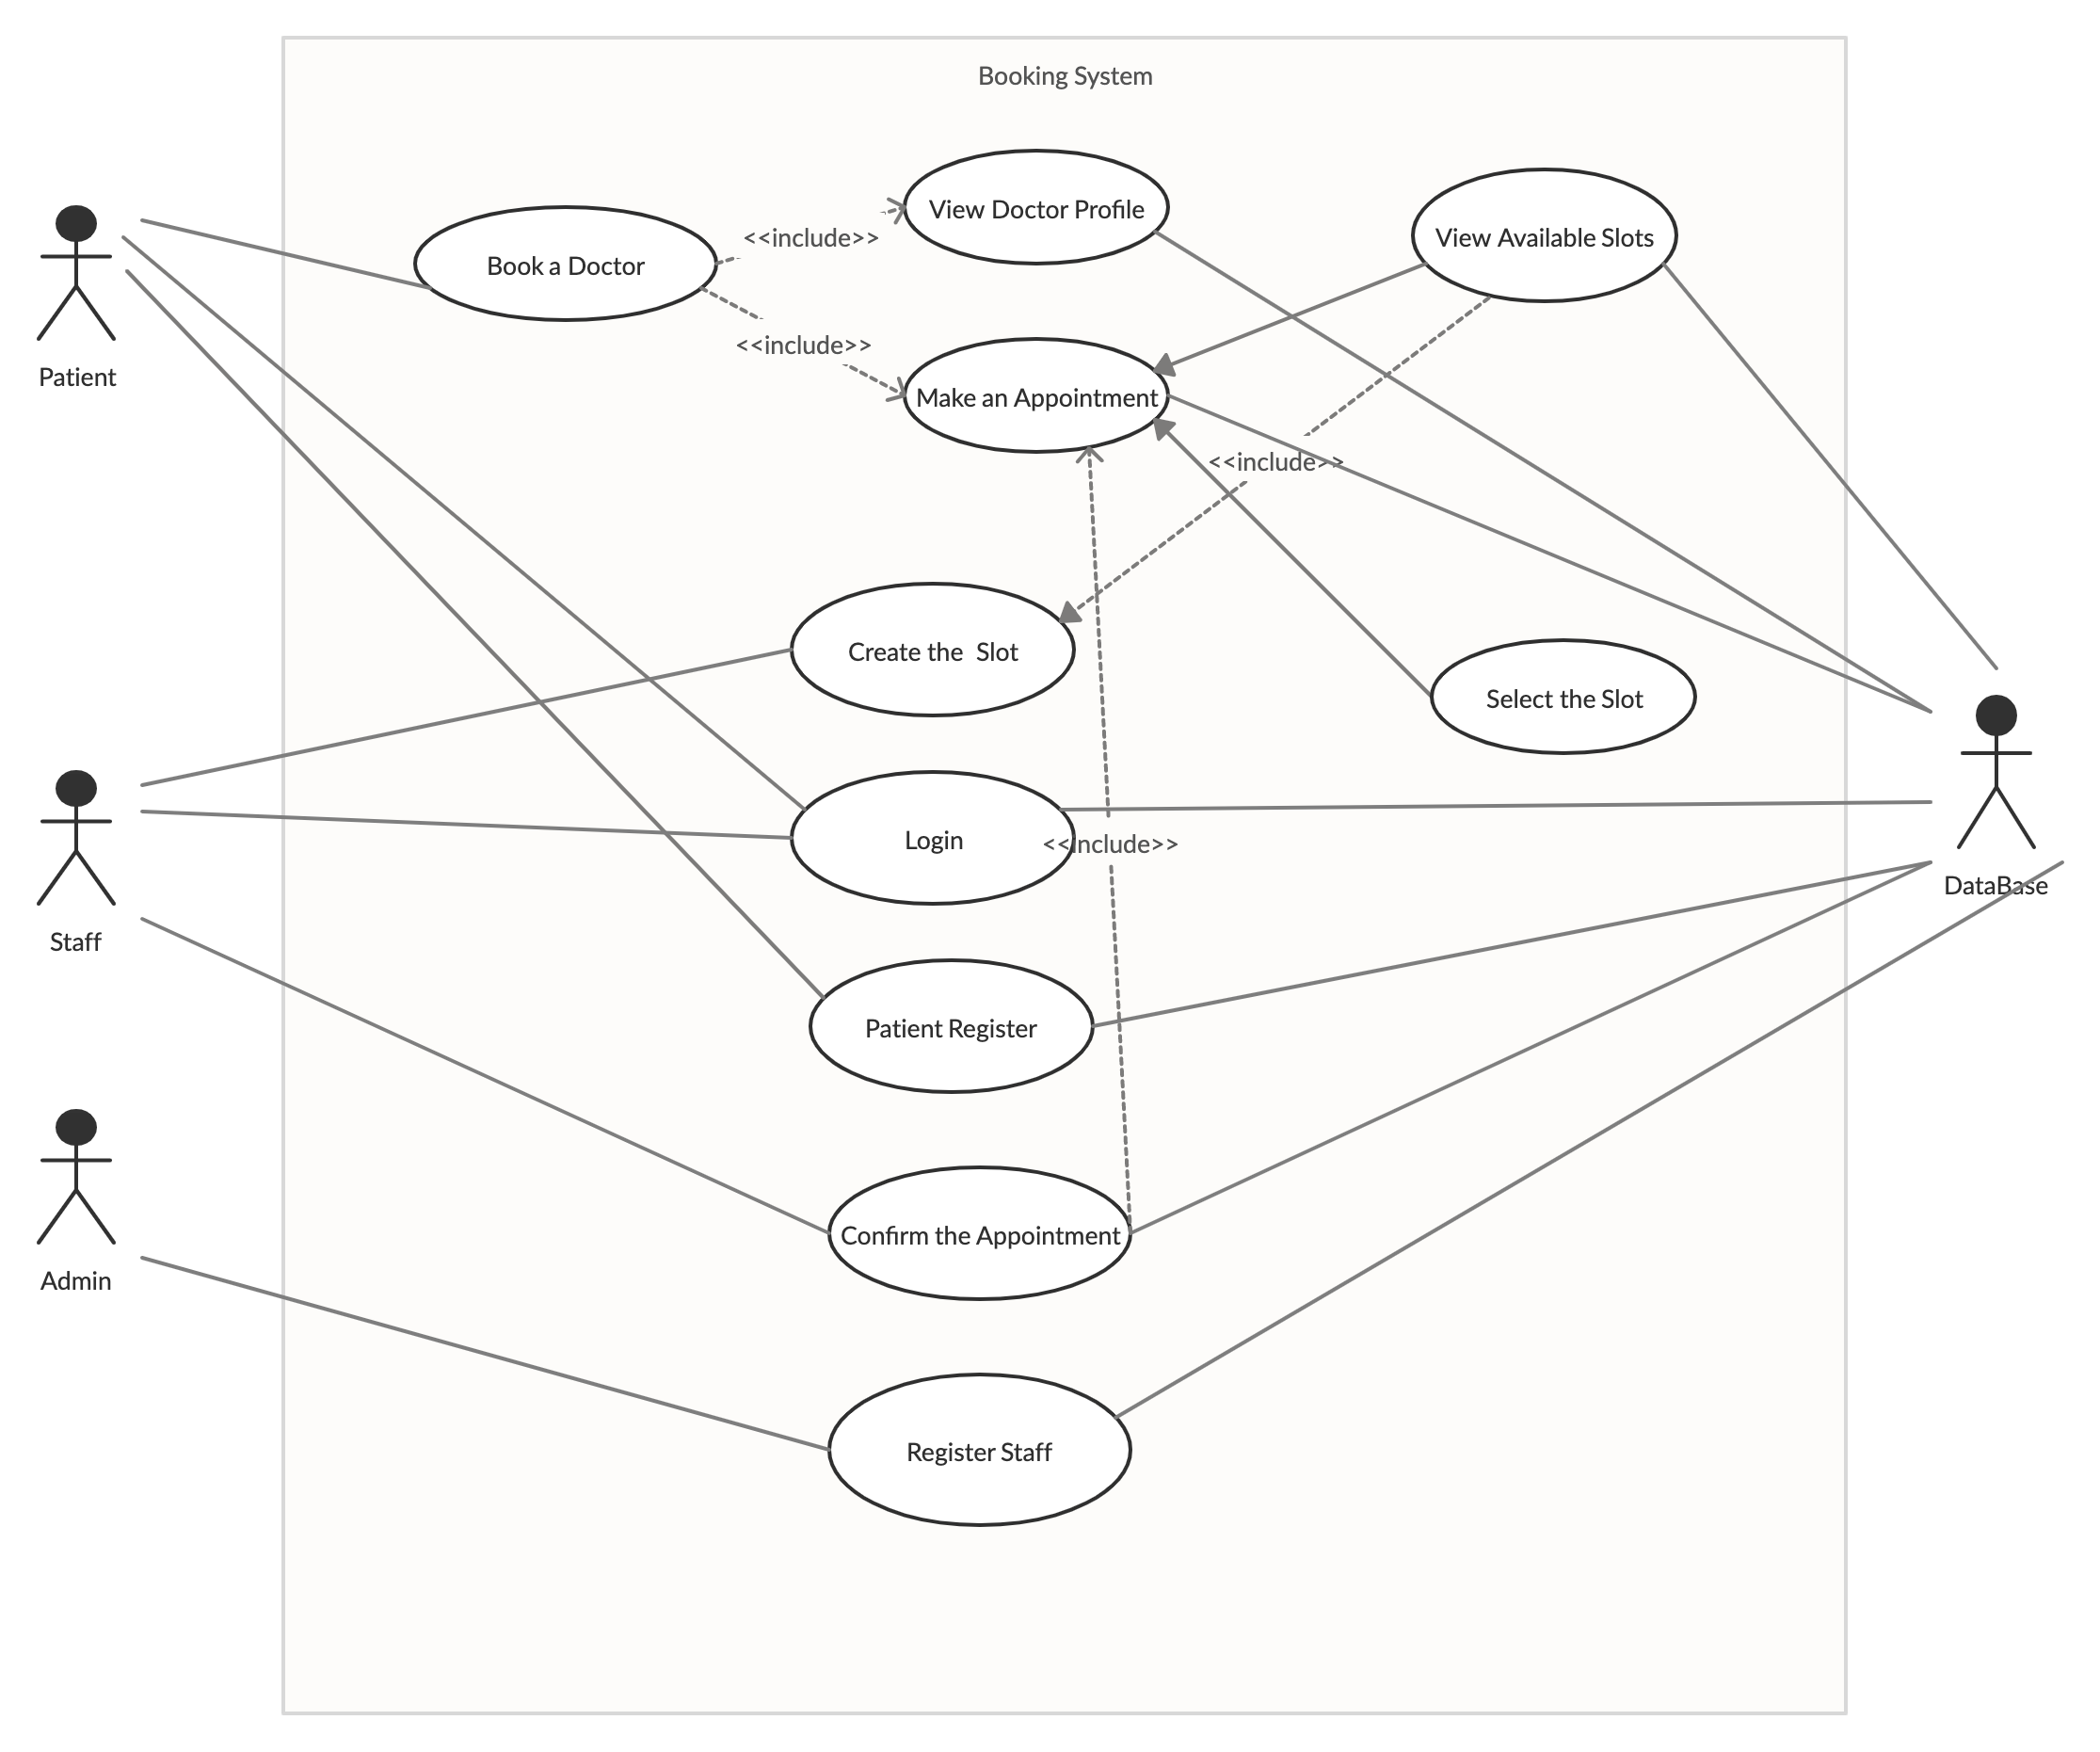
\includegraphics[scale=.15]{UML/UseCase.png}\\
        \textbf{Use Case Diagram}
        \addcontentsline{lof}{section}{Use Case Diagram}
    \end{center}
    
    \begin{center}
        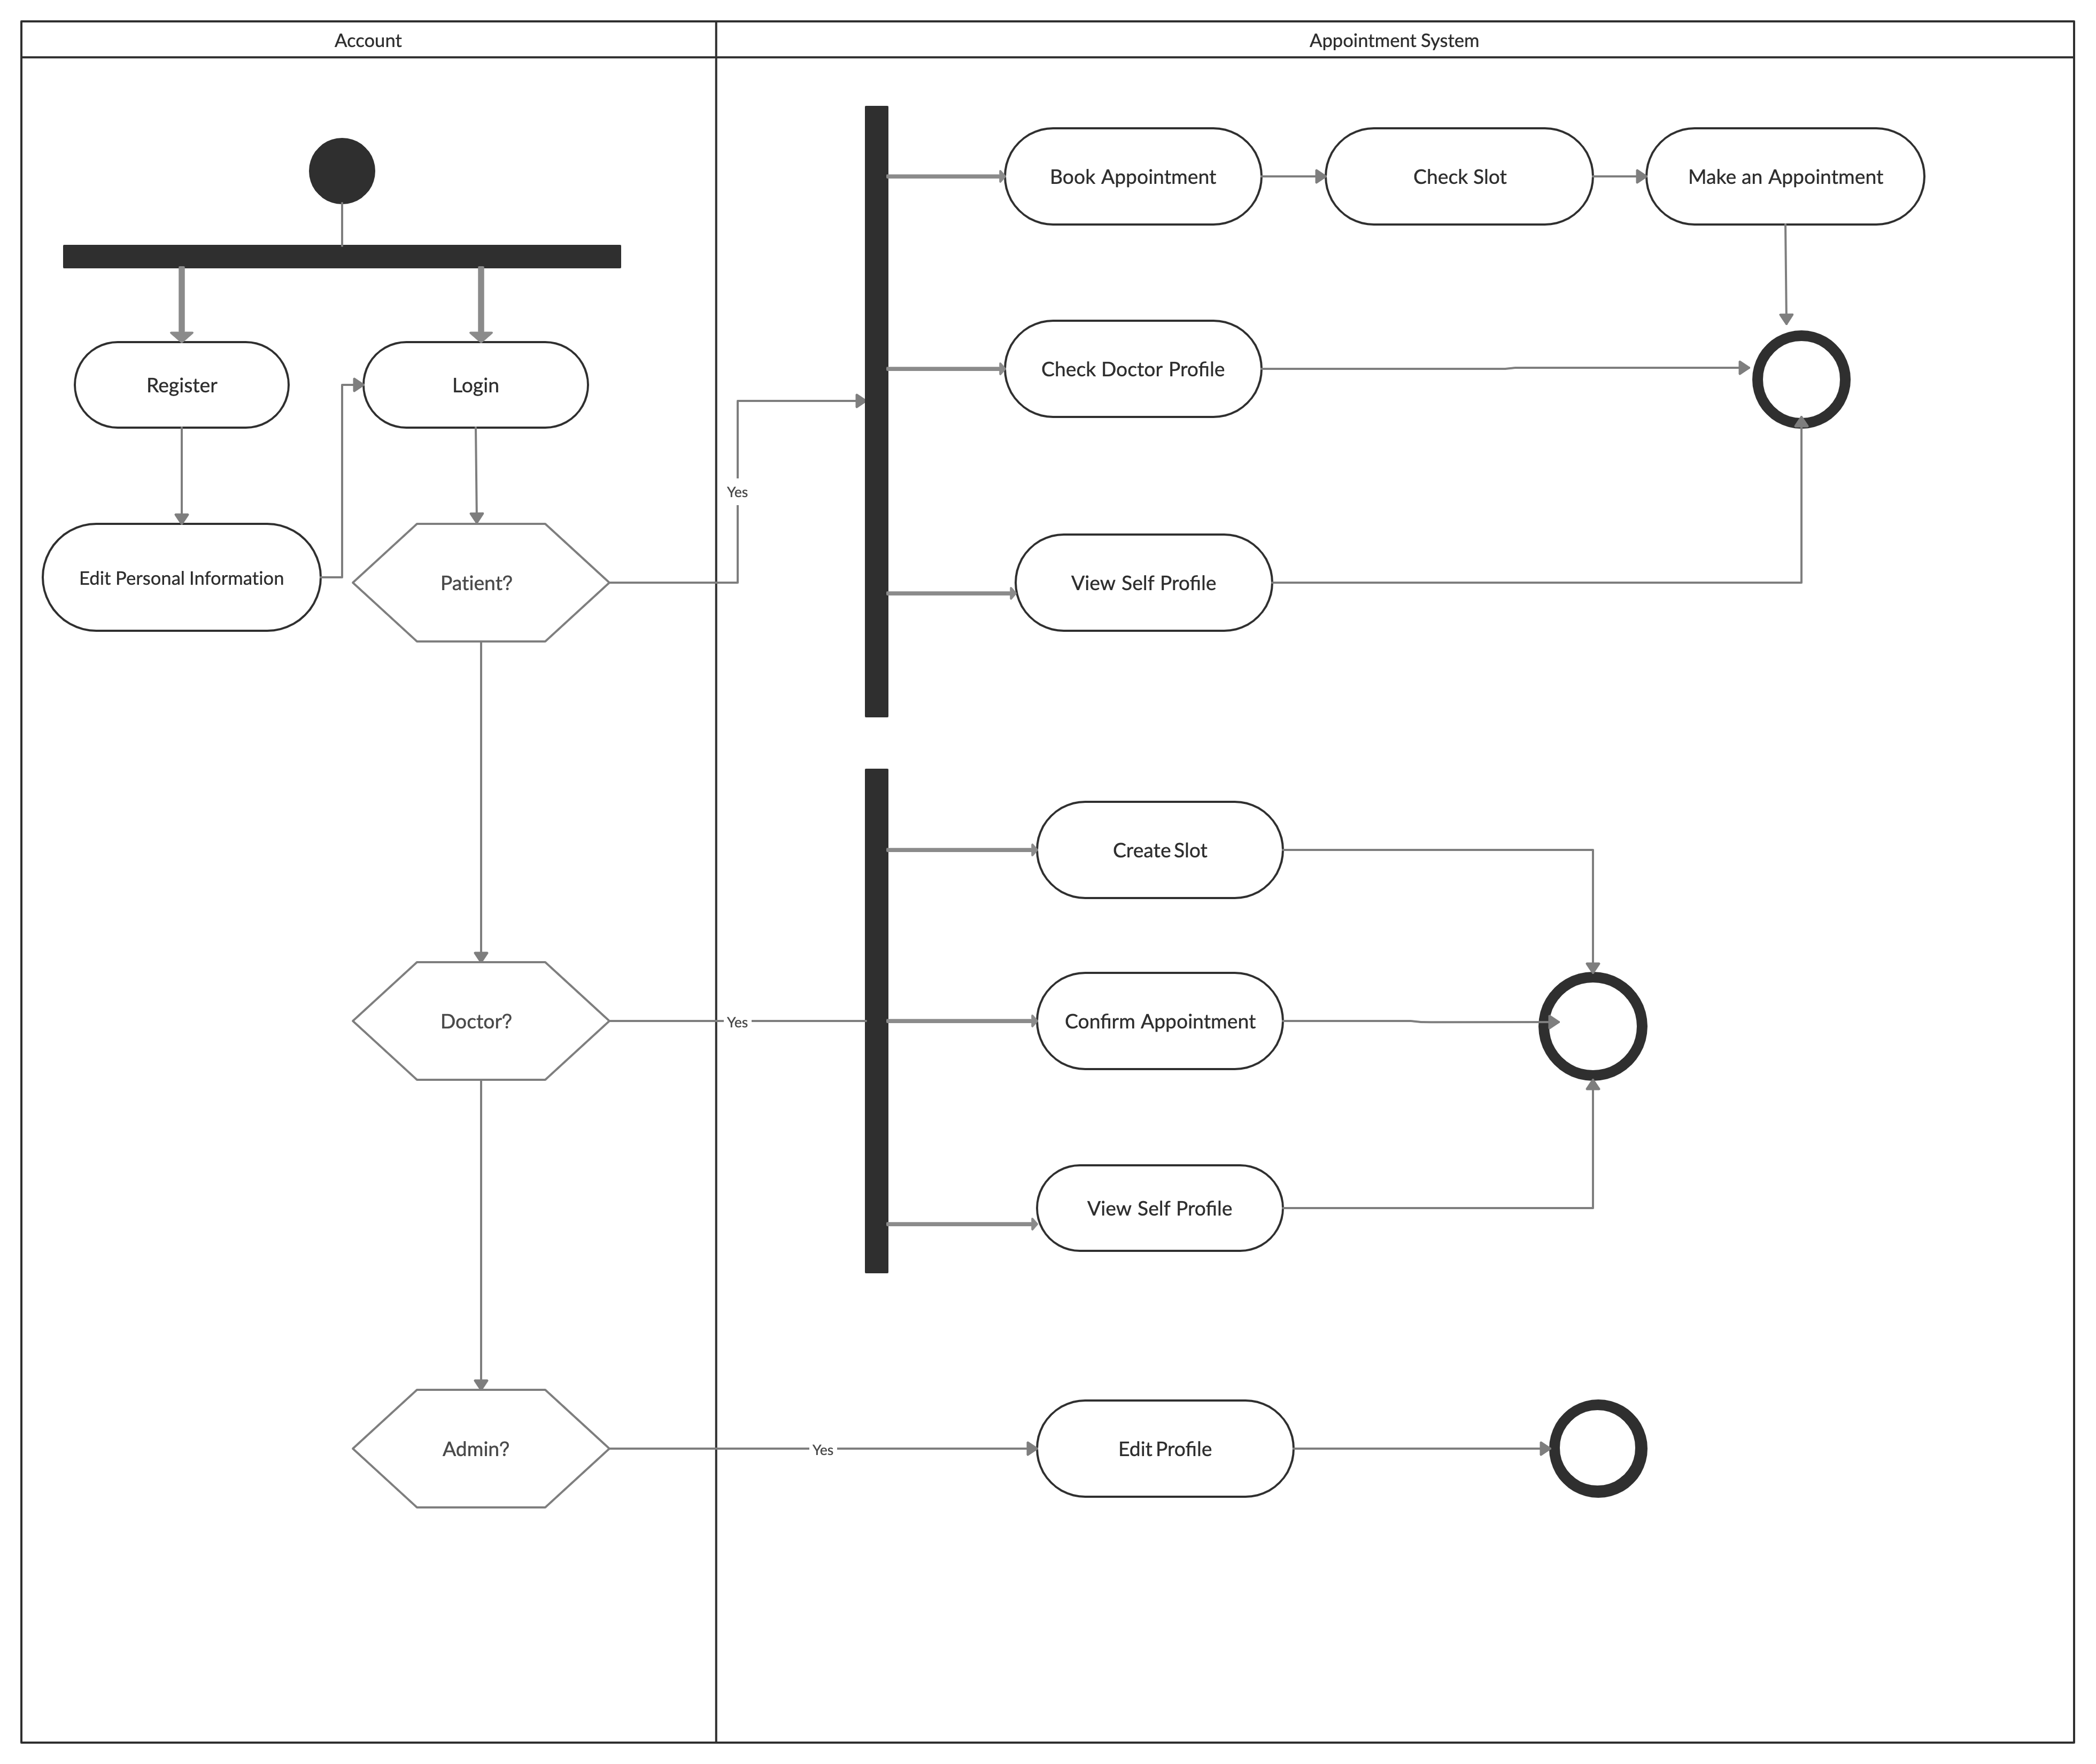
\includegraphics[scale=.1]{UML/activity.png}\\
        \textbf{Activity Diagram}
        \addcontentsline{lof}{section}{Activity Diagram}
    \end{center}
    
\addcontentsline{toc}{chapter}{PART 5: ARCHITECTURAL DECISIONS}

\chapter*{PART 5: ARCHITECTURAL DECISIONS}

\addcontentsline{toc}{section}{Architectural Decision 1: Use the MVC architecture}
\section*{Architectural Decision 1: Use the MVC architecture}
The PHP development model mixes the code of data access, the processing of business logic, and web presentation layer together, as a result, it brough about many problems in the web applications[cite]. In ICARE project, there are three types of users, namely patient, staff and administrator, and different users play different roles in the system. So it is essential to divide these users into different models. 

\begin{enumerate}
    \item \textbf{Decision:} 
    \newline\newline We will organize ICARE with the MVC pattern.
    
    \begin{enumerate}
        \item{\textbf{Rationale:}}  
        \newline\newline The knowledge acquired in industrial and academic experiences \textbf{[02]} \textbf{[03]} shows that using patterns (specifically, architectural patterns) in systems development allows (1) discerning the domain where the system is being developed, (2) satisfying systemic properties (“quality attributes” or QAs \textbf{[04]}), and (3)creating large-scale reuse design techniques (frameworks \textbf{[05]}). In ICARE, initially, the user interact with the login in page and then the system show corresponding page according to the role of the user. So it is clear that the front page is a controller and view will get the data from model to show in the website. The MVC pattern is abstracted into three parts as model, view, and controller. Model interact with database systems (or simply data storage systems) and responds to request of data (usually from view). Controller responds to events (click  of  mouse, keyboard stroke etc.) and informs model and/or view to make changes accordingly \textbf{[06]}. The view is the application interface shown or seen by the clients and interacts with the clients. A view will be loaded in the browser by the controller according to the client’s request \textbf{[07]}.
    \end{enumerate}
    
    \item \textbf{Status:} 
    \newline\newline Accepted
    
    \item \textbf{Consequences:} 
    
    \begin{center}
        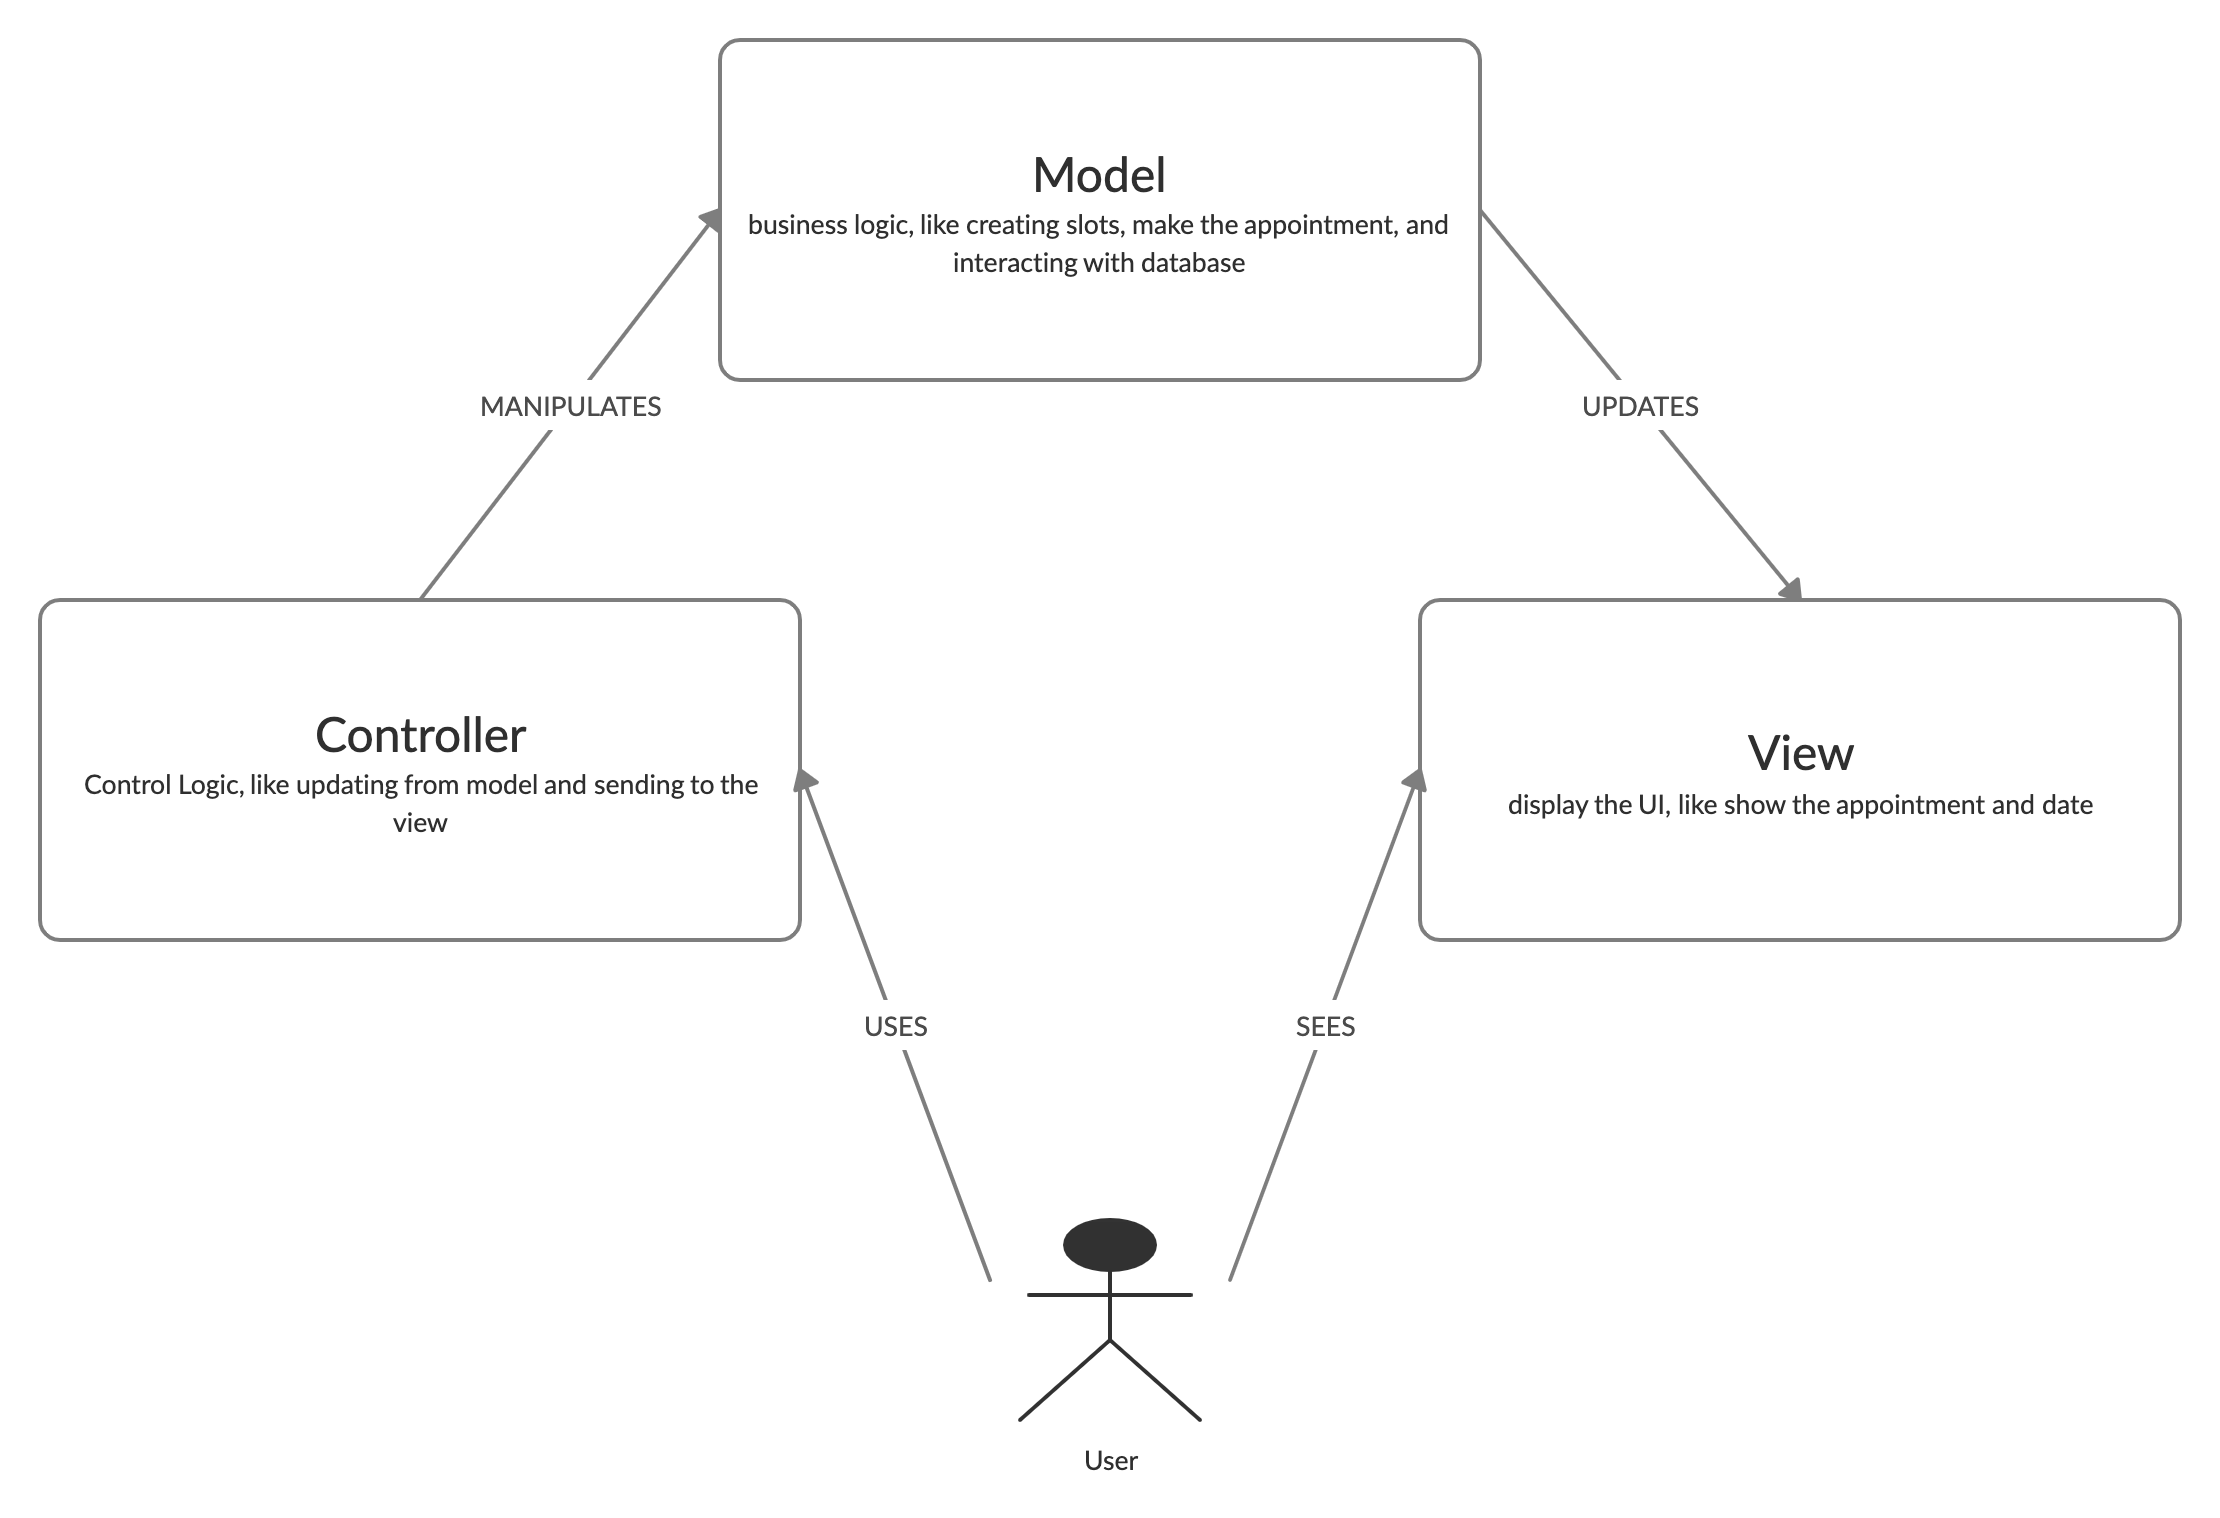
\includegraphics[scale=.2]{UML/MVC.png}\\
        \textbf{MVC Pattern for ICARE}
        \addcontentsline{lof}{section}{MVC Pattern for iCARE}
\end{center}

    ICARE is to follow the MVC pattern. The front controller will response to the users' click and filling conduct when login/ signing up. The controller calls the model to complete the read-write operation including viewing profile and make the appointment.The View will show the data in the web browser. 
\end{enumerate}
 
 
 
\addcontentsline{toc}{section}{Architectural Decision 2: Architectural tactics}
\section*{Architectural Decision 2: Architectural tactics}
Software architectural tactics are a group of design decisions that influence quality attributes to transform a software design’s behaviour. In spite of architectural patterns, which include trade-offs, tactic focus on specific quality attributes, and it does not consider trade-offs (should be considered by the designer).

\begin{enumerate}
    \item \textbf{Decision:} Regarding using the MVC pattern, we choose the following:
    
    \begin{enumerate}
        \item \textbf{Security tactics:}
        \begin{enumerate}
            \item \textbf{Authentication users (Resisting Attacks) tactic:} It ensures a user or remote computer is actually who it purports to be. Passwords, one-time passwords, digital certificates, and bio-metric identifications provide authentication.
            
            \item \textbf{Authorize Users (Resisting Attacks) tactic:} By allowing just the users who are allowed to modify or access specific data.
            
            \item \textbf{Intrusion detection (Detecting Attacks) tactic:} Detecting an ongoing attack is vital to be ready to react and reduce its consequences.
        \end{enumerate}
    
        \item \textbf{Safety Tactics:}
        \begin{enumerate}
            \item \textbf{Simplicity (Failure Avoidance) tactic:} By making the software simple we tried to reduce faults.
            \item \textbf{Timeout (Failure Detection) tactic:} By assuming there would be failures in any software system, the timeout tactic would help to detect a possible failure.
        \end{enumerate}
        
        \item \textbf{Modifiability Tactics:}
        \begin{enumerate}
            \item \textbf{Increase semantic cohesion tactic:} Separates user interface responsibilities from the co-functionality of the system, so all the views can reside in common components.
            \item \textbf{Using intermediary tactic:} Controllers are used as intermediaries between view and the data to break dependencies between view and the model.
            \item \textbf{Run-time binding:} By deferring bindings time to run-time, they can be changed when the program is running.
        \end{enumerate}
    \end{enumerate}
\end{enumerate}

\addcontentsline{toc}{section}{Architectural Decision 3: Principles}
\section*{Architectural Decision 3: Principles}
MVC Architecture or Model View Controller Architecture basic principle is to divide the system into logic of the system and presentation of the system to make the system more maintainable. Hence the system is divided into 3 parts: 

\begin{enumerate}
    \item \textbf{View:} The presentation part of the system is in the View. The user will just interact with the view and will not be able to interact with any other part of the system. In iCare, the patient will be able to access this section when they use the login module, appointment booking, viewing doctor profile, viewing reports and such others. Similarly, the staff or doctor can view patient’s profile, view booking schedule, reschedule appointments, and so on. Hence, basically, any interaction including the user input, viewing the system by the user is all processed through the view of the system and it also responsible for giving an appropriate response based on the input.
    
    \item \textbf{Model:} It possess the logic of the system. The input obtained from view is controlled by the controller, processed, and passed to the model which then update the state of the system accordingly. The state of the system is managed by model and every time the state of the system is manipulated with the change in the input. For example, when the user clicks on the ‘Sign-in’ button to login, the data from the View are managed by the model and the state is updated by model.
    
    \item \textbf{Controller:} It controls the above Model and View. The controller manages the data between the model and view. The data obtained from the user by the view is processed by the controller and passed on to the model to update the state of the system. Once, the model changes the state, the controller process that and an appropriate view is called by the controlled and view show that as a response to the user input.
\end{enumerate}


\addcontentsline{toc}{section}{Architectural Decision 4: Styles }
\section*{Architectural Decision 4: Styles}
\begin{center}
    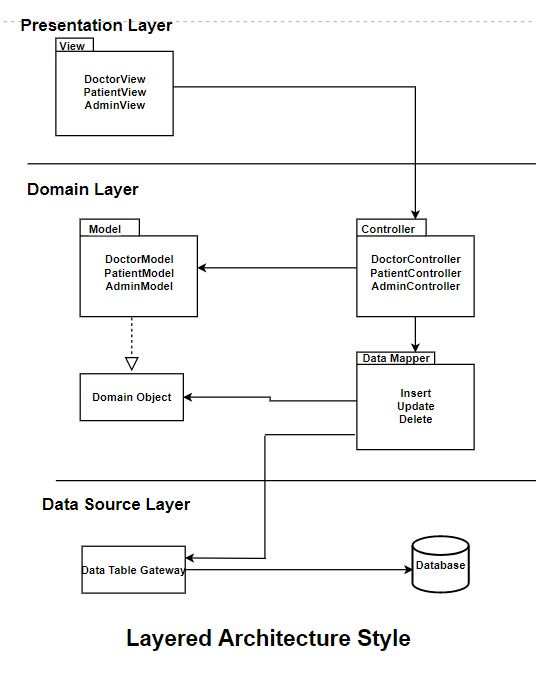
\includegraphics{UML/LayeredArchitectureStyle.JPG}
    \addcontentsline{lof}{section}{Layered Architecture Style}
\end{center}
Layered architectural style, otherwise known as n-level engineering style, it is one of the most widely recognized styles utilized in the software development life cycle.  Icare application is following layered architecture. A presentation layer would be responsible for managing all user interface and browser communication logic, while a domain layer would be responsible for enforcing specific business rules pertaining to a request. The presentation layer does not need to know or worry about how to get doctors, patient data; it only needs to display that information on a screen format. Similarly, the domain layer does not need to be concerned about how to format doctors, patient data for display on a screen or even where the doctors, patient  data is coming from, it only needs to get the data from the data source layer, perform business logic against the data and pass that information up to the presentation layer.  In the event that a patient’s needs to book an appointment, he will initially need to interact with the presentation  layer(Book appointment form), which is the top-most layer , the main function of this layer is to translate tasks and results to something the patient  can understand. And afterward the patient request is handled by middle layer which is called domain layer(bookingController). It is used to coordinate to application layer and makes logical decision by patient request. Domain layer will validate the data received from booking form and then it goes to data source layer, which has a control to the actual database, to perform the database writing.


\addcontentsline{toc}{chapter}{PART 6: IMPLEMENTATION}
\chapter*{PART 6: IMPLEMENTATION}

\section*{Tools and Technologies:}
\begin{enumerate}
    \item \textbf{Tools:} 
    \begin{enumerate}
        \item Sublime Text Editor
        \item Wamp Server(LocalHost)
        \item Google Chrome
        \item draw.io
        \item creately.com
        \item XMind
    \end{enumerate}
    
    \item \textbf{Technologies:} 
    \begin{enumerate}
        \item php
        \item Bootstrap 4
        \item MySQL
        \item HTML
        \item CSS
        \item Javascript
        \item Ajax
    \end{enumerate}
\end{enumerate}

\section*{Homepage:}
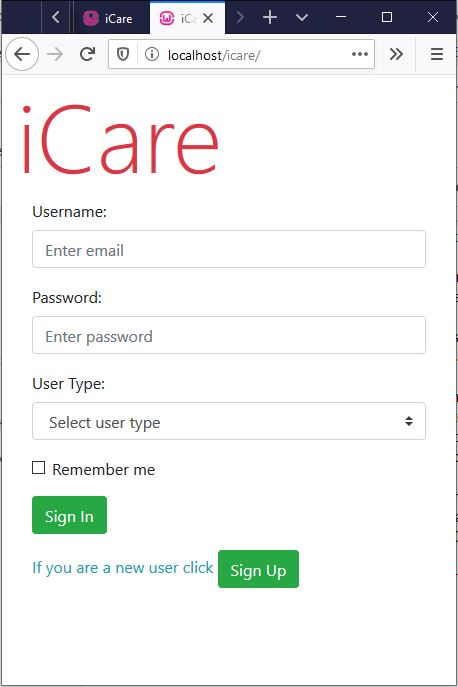
\includegraphics[scale=0.8]{Implementation/homepage.JPG}
\addcontentsline{lof}{section}{Homepage}

\section*{Patient Sign Up:}
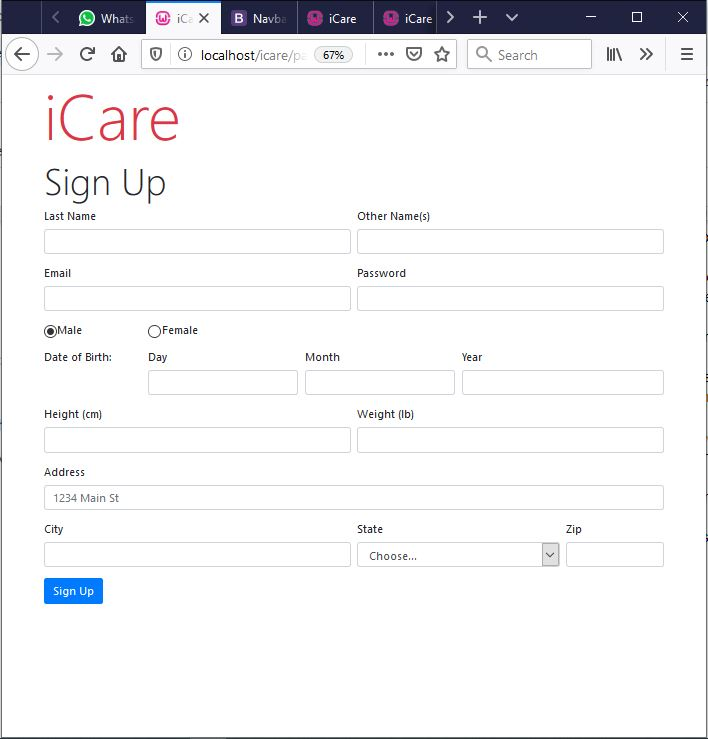
\includegraphics[scale=0.8]{Implementation/patientSignUp.JPG}
\addcontentsline{lof}{section}{Patient Sign Up}

\section*{Patient Dashboard:}
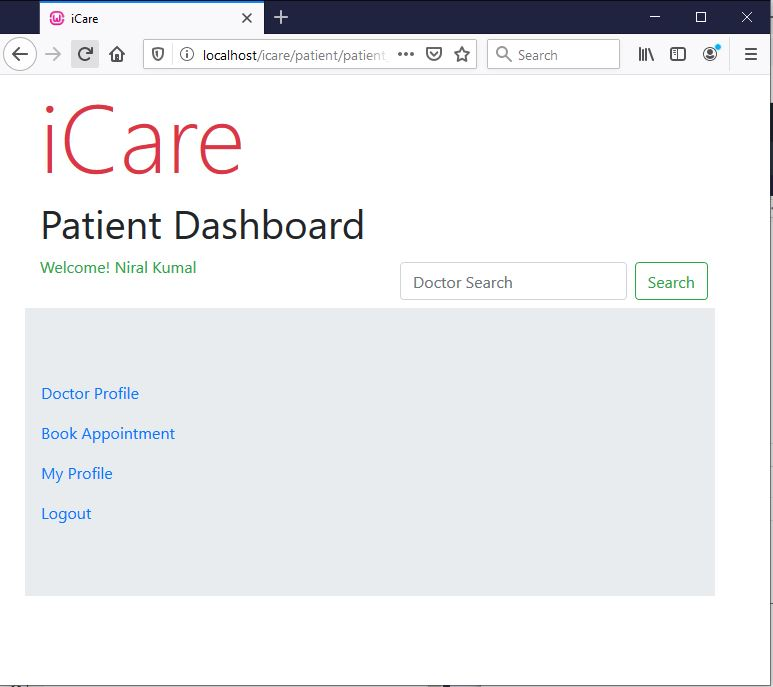
\includegraphics[scale=0.8]{Implementation/patientDashboard.JPG}
\addcontentsline{lof}{section}{Patient Dashboard}

\section*{Book Appointment:}
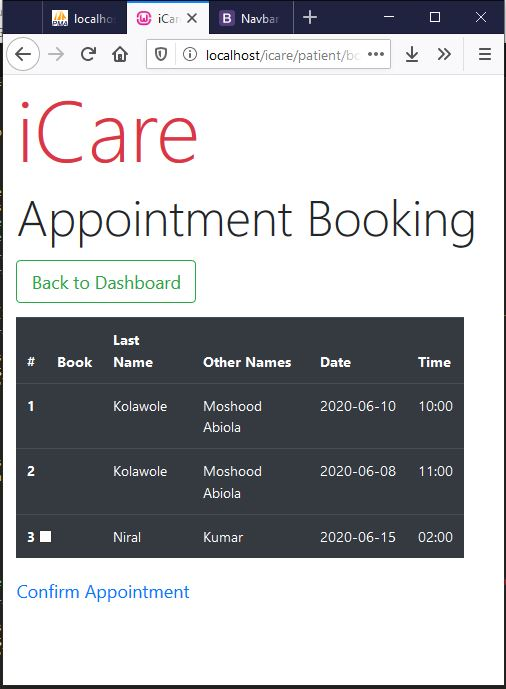
\includegraphics[scale=0.8]{Implementation/bookAppointment.JPG}
\addcontentsline{lof}{section}{Book Appointment}

\section*{Doctor Profile:}
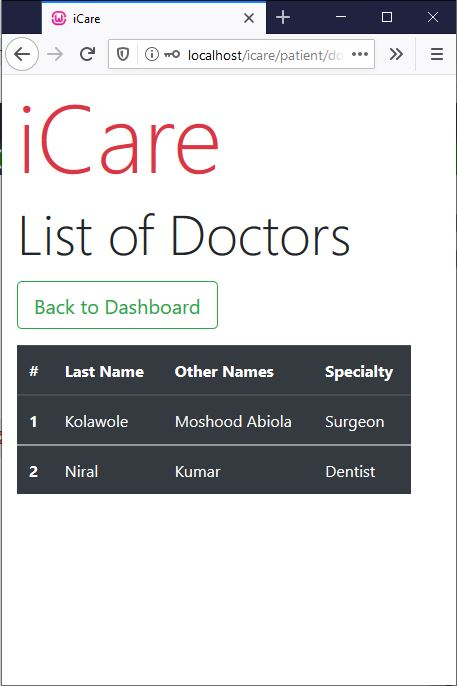
\includegraphics[scale=0.8]{Implementation/doctorProfile.JPG}
\addcontentsline{lof}{section}{Doctor Profile}

\section*{Doctor Dashboard:}
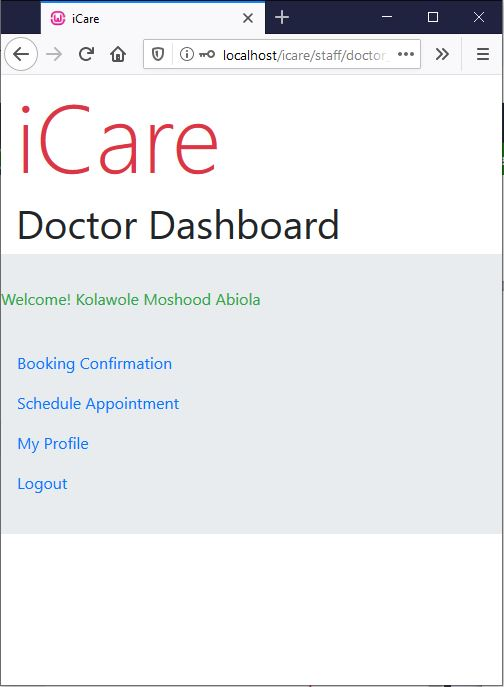
\includegraphics[scale=0.8]{Implementation/doctorDashboard.JPG}
\addcontentsline{lof}{section}{Doctor Dashboard}

\section*{Staff Registration:}
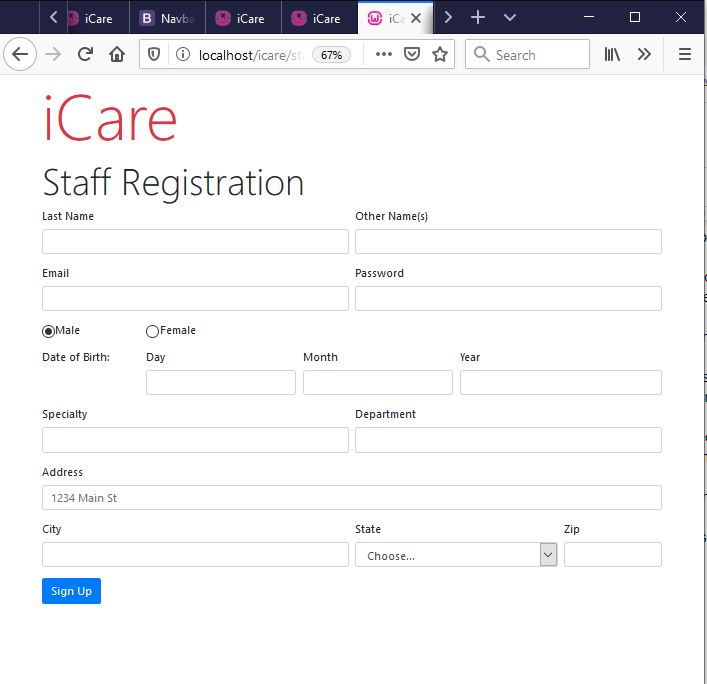
\includegraphics[scale=0.8]{Implementation/staffRegistration.JPG}
\addcontentsline{lof}{section}{Staff Registration}

\section*{Schedule Appointment:}
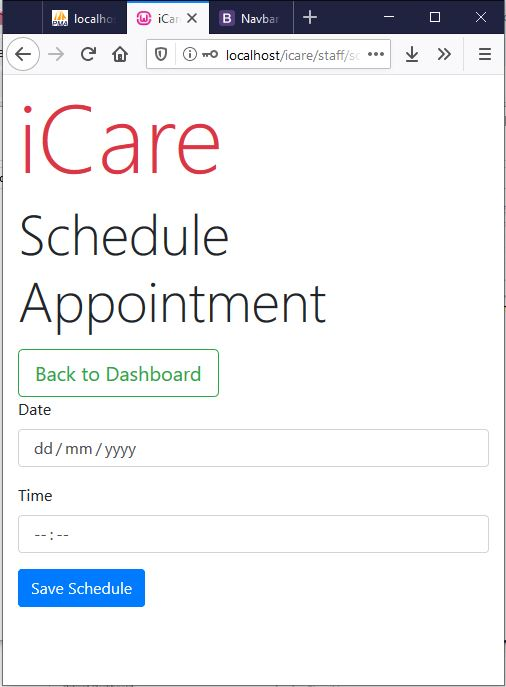
\includegraphics[scale=0.8]{Implementation/scheduleAppointment.JPG}
\addcontentsline{lof}{section}{Schedule Appointment}

\section*{Admin Dashboard:}
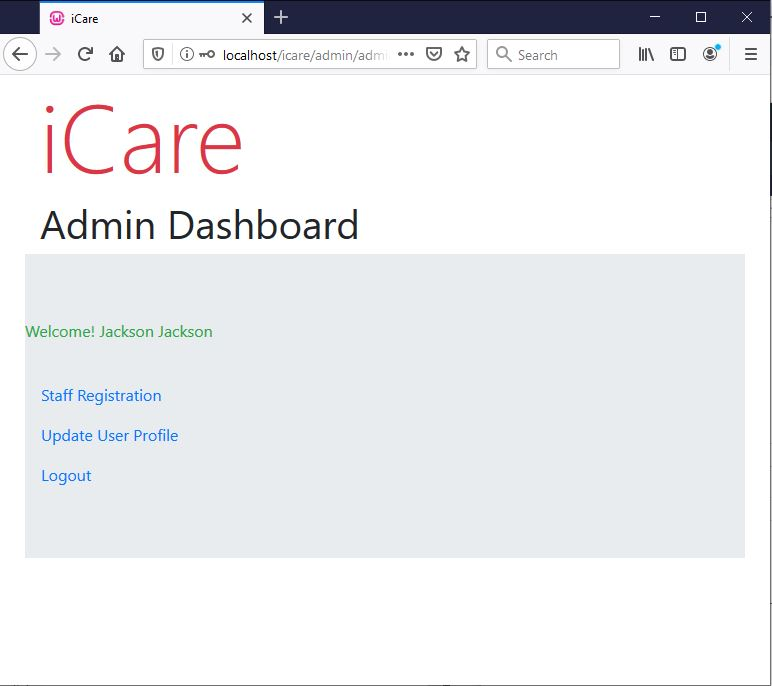
\includegraphics[scale=0.8]{Implementation/adminDashboard.JPG}
\addcontentsline{lof}{section}{Admin Dashboard}

\addcontentsline{toc}{chapter}{REFERENCES}
\chapter*{REFERENCES}

\begin{enumerate}
    \item Concordia University Logo: \url{https://www.google.com/search?q=concordia+university+logo&sxsrf=ALeKk00nNpzxCfTcJxEwAQNk-ilil0DPkg:1591909168136&tbm=isch&source=iu&ictx=1&fir=Ccxmok0d1jX1RM%253A%252C01bcPIzeDtiMbM%252C_&vet=1&usg=AI4_-kS2jmerHVUL2zX5hpT8LOFsJhz51w&sa=X&ved=2ahUKEwiey-zj0_rpAhVNRjABHXHQDfAQ9QEwAHoECAsQIw&biw=1366&bih=625#imgrc=fzpIxbXYP_q83M}
    
    
    \item
    M. Fowler,Patterns of Enterprise Application Architecture. Boston, MA,USA: Addison-Wesley Longman Publishing Co., Inc., 2002.
    
    \item
    M. Kircher and J. Prashant, Pattern-Oriented Software Architecture.Patterns for Resource Management. West Sussex, England: Wiley seriesin software design patterns, 2004.
    
    \item L. Chung, B. A. Nixon, E. Yu, and J. Mylopoulos, Non-functionalrequirements in software engineering, vol. 5.  Springer Science andBusiness Media., 2012.
    
    \item R. E. Johnson, “Frameworks = (components + patterns),”Commun.ACM, vol. 40, no. 10, pp. 39–42, 1997.
    
    \item 
    Aditya Singh, Piyush Chawla, Karan Singh, Ashutosh Kumar Singh, Formulating an MVC Framework for Web Development in JAVA \url{https://ieeexplore-ieee-org.lib-ezproxy.concordia.ca/stamp/stamp.jsp?tp=&arnumber=8553746}
    
    \item 
    Stenly Ibrahim Adam, Stevani Andolo, A New PHP Web Application Development Framework Based on MVC Architectural Pattern and Ajax Technology\url{https://ieeexplore-ieee-org.lib-ezproxy.concordia.ca/stamp/stamp.jsp?tp=&arnumber=8874912}
    
    \item \url{https://www.student.cs.uwaterloo.ca/~cs446/1171/Arch_Design_Activity/Layered.pdf}
    
     \item \url{https://users.encs.concordia.ca/~cc/soen6461/}
    
    \item \url{https://creately.com/diagram/example/indonknf1/New%20Patient%20Appointment%20System}
     
     \item \url{https://www.htmlgoodies.com/beyond/php/article.php/3912211/Principles-Of-MVC-for-PHPDevelopers.htm#:~:text=MVC%2C%20or%20Model-View-,be%20separated%20from%20its%20presentation.}
    
     \item  Bass, L., Clemens, P., Kazman, R.: Software Architecture in Practice. SEI Series in Software Engineering, Addison-Wesley, 2 edn. (2003)
     
     \item Schumacher, M., Fernandez-Buglioni, E., Hybertson, D., Buschmann, F., Sommerlad, P.: Security Patterns: Integrating Security and Systems Engineering. John Wiley and Sons (2006)
     
     \item Wu, W., Kelly, T.: Safety Tactics for Software Architecture Design. In: Proc. 28th Annual International Computer Software and Applications Conference COMPSAC 2004. pp. 368–375 (2004)
    
\end{enumerate}


\end{document}

